\documentclass[10pt]{article}
\usepackage[T1]{fontenc}
\usepackage{lmodern,amsmath,amssymb,graphicx,hyperref}
\usepackage[margin=.75in]{geometry}
\setlength{\parindent}{0pt}\setlength{\parskip}{7pt}
\begin{document}
\begin{center}{\Large Actual absolute-precision coefficient transport}\\[5pt]
14 November 2026; 53 authored statements\\
\texttt{eedce945208bf58a980e3e133bd11c9b135f3e6a}
\end{center}

\textbf{Checked component.} The isolated source has53 authored statements:
12 copied historical mode statements and41 newly bound declarations. The
pinned shared gate audits57 declarations with0 extra trusted axioms, exit0.
The owned project builds without warnings. Import-inclusive fresh replay
is running; no completed pass is claimed. All records remain unsigned,
defaultnot\_covered [pcc:unverified].

\textbf{Same actual family.} Keep the existing auxiliary completed $W$ and its
explicit crossing mask. Use actual ports $x,y<2^a$, a nonzero signed-grid node
$t$ with $v_2(t)=i<u\le a$, natural multiplicities and actual feasible
schedule $G_i\ge0$. The negative-pole diagonal scalar has weight
$w=a+1-i+G_i\ge2$. No favorable local first jet or new origin is supplied.

For an absolute creation precision $p\in\mathbb N$, construct
\[
 k=\operatorname{toNat}(p-w),\qquad w+k\ge p,\qquad k\le p.
\]
Actual left/right polynomial factors satisfy
\[
 \begin{gathered}
 \operatorname{Content}_{w+b}(A_{x,(r,b)}),\quad
 \operatorname{Content}_0(B_{(r,b),y}),\quad
 \deg B_{(r,b),y}\le p,\\
 \operatorname{Content}_{p}(W^{\rm cross}_{xy}-(AB)_{xy}),\quad
 (r,b)\in[2^u]\times[k],\quad \#\text{labels}\le2^u p.
 \end{gathered}
\]
The case $k=0$ is retained. All literal labels remain charged; the displayed
bound is a declared inventory bound, not a nonzero-mode count or runtime
estimate [pcc:unverified].

\begin{center}
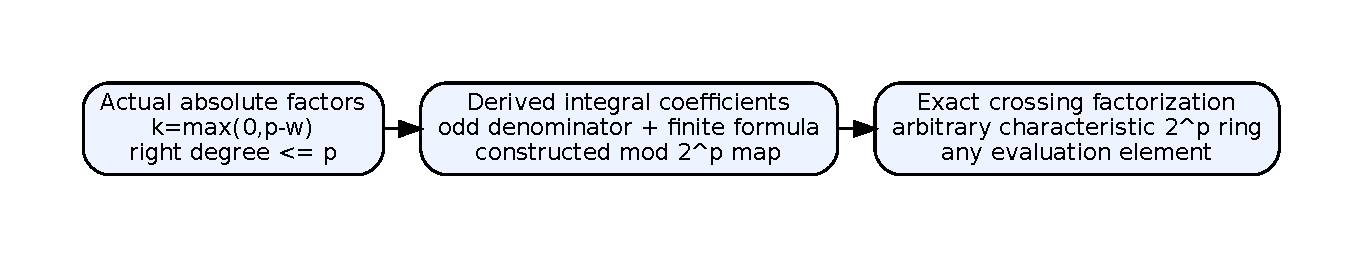
\includegraphics[width=\linewidth,height=1.25in,keepaspectratio]{dependencies.pdf}
\end{center}
\textbf{Result after coefficient transport.} Construct integral coefficient
lifts of these actual matrices. Their reductions factor exactly over every
commutative ring of characteristic $2^p$, and the identity survives evaluation
at every element of that ring, including nilpotents. Integrality of the
actual $W$ coefficients is derived from its actual residual and integral
product, rather than assumed as a favorable witness [pcc:unverified].

\newpage
\begin{center}{\Large Actual coefficient map and source bindings}\end{center}
Define the actual subring
\[
 I=\{q\in\mathbb Q:q=0\text{ or }v_2(q)\ge0\}.
\]
The construction uses the standard embedding $I\to\mathbb Z_2$ and Mathlib's
canonical homomorphism $\mathbb Z_2\to\mathbb Z/2^p\mathbb Z$. It proves
the reduced denominator of each $q\in I$ is odd. Thus the map also has the
finite formula
\[
 \rho_p(q)=\operatorname{num}(q)\,
                 \operatorname{den}(q)^{-1}\pmod{2^p},
\]
with the denominator's unit property derived from actual integrality.
It proves $\operatorname{VBound}_p(q)\Rightarrow\rho_p(q)=0$ and coherent
downward precision reduction. No favorable homomorphism or odd-denominator
premise is supplied by the caller [pcc:unverified].

Finite-support coefficient lifts map back to the exact rational polynomials.
Coefficientwise content-$p$ error therefore maps to the zero polynomial.
Finite matrix sums/products commute with this coefficient homomorphism;
ordinary polynomial evaluation then gives exact factorization at any
target-ring element. The characteristic-$2^p$ target ring is explicit in the
theorem statement. This does not construct the original unramified extension
data or its computational representation [pcc:unverified].

\begin{center}\small
\begin{tabular}{p{.66\linewidth}p{.24\linewidth}}
\texttt{actual\_absolute\_polynomial\_precision}&PCC-20261114-27c970\\
\texttt{actual\_absolute\_rational\_profile}&PCC-20261114-fd920f\\
\texttt{reduce\_compatible}&PCC-20261114-595bad\\
\texttt{reduce\_finite\_formula}&PCC-20261114-00399c\\
\texttt{actual\_reduced\_absolute\_factors}&PCC-20261114-05dd71\\
\texttt{actual\_evaluated\_absolute\_profile}&PCC-20261114-a97a53
\end{tabular}
\end{center}
All41 exact source bindings are in
\begin{center}\small
\path{../evidence/claim-pins.json}\\
\path{../evidence/source-freeze.json}\\
\path{../evidence/gate-validation-001.json}.
\end{center}
Gate data is PCC-20261114-36928e. The12 copied historical mode declarations
are covered by the new module's shared audit but are not reissued as new
claims. Four generated declarations are listed in the gate receipt. All
standing remains unsigned/defaultnot\_covered [pcc:unverified].

\newpage
\begin{center}{\Large Validation and original cost interface}\end{center}
\textbf{Pinned environment.} Lean4.35.0; CryptoLean and Mathlib revisions:
\begin{center}\small
\texttt{148f5dc389b341401e06d76abe7783c4ccf42f2e}\\
\texttt{cfc55fc58714a59dc06e6e79edc6d1d95140d3c2}.
\end{center}
The accepted local draft015 is copied byte for byte. Shared gate57/0 and
owned build0 are complete; import-inclusive
\texttt{leanchecker --fresh --verbose OrientationTransport} is pending.
Local acceptance is not substituted for that replay [pcc:unverified].

All failed local drafts/raw logs are retained: module-header/import visibility,
subtype/norm casts, finite-support wrapper and exported reduction requirements,
matrix extensionality and namespace/indentation failures. No warning, premise,
test or gate was disabled. Old Degree108+final15, Compact106+final13,
Higher83+final13 and Node90 pins remain exact. Degree's completed fresh report
and explicit40-to41-byte claim correction remain independently versioned
[pcc:unverified].

\textbf{Original mode cost remains separate.} The primary D.12--16 interface
uses $2^{i+1}$ column tiles, at most $6M/D_i$ modes per weight, one source
and target group per mode, and immutable creation-precision descriptions.
The current construction charges every $2^u$ row class per moment. Its
absolute degree bound and finite coefficient formula do not count the bit
operations for coefficient construction or weighted child extraction.

Downward coherence of $\rho_p$ is not an immutable canonical lift to a larger
precision. A creation-time residue is represented once; reevaluating its old
rational formula at a new precision can change that representative. The
original primary text explicitly avoids treating canonical lifting as a
ring homomorphism. This interface must be charged and connected separately
[pcc:unverified].

\textbf{Next accounting.} Bound actual numerator/denominator sizes and entry
work at creation precision; preserve immutable descriptions; charge mode
inventory, coefficient extraction, child networks, recovery and every
recursive call. Actual elliptic relation/public finder, field/scalar
extraction, retries and complete expected bit cost remain open. No algorithm
or runtime exponent follows from this component [pcc:unverified].

\textbf{Sources checked.} KB unavailable as journaled. Read exact LocalIntegral,
Degree/Compact/Higher/Node source and pinned Mathlib PadicVal.Basic,
PadicIntegers, RingHoms and polynomial/Finsupp/monoid-algebra APIs. Re-read
primary D.4.6 and the repository contraction-precision review. Standard
p-adic reduction and matrix algebra are reused without novelty, priority,
fastest-method or timing claim.

No new native, attack, paid/cloud or F4/msolve/timing/scaling campaign.
The original norm fixture remains unlaunched under its transport blocker.
Protected ledger divergence remains an integration prerequisite requiring
the canonical maintainers' supported reconciliation contract; auto-merge
stays off. No rechain, trust/signature or prefix waiver [pcc:unverified].
\end{document}
